%% Final report, COL7761 (ICTD), IIT Delhi.
%% ACM two-column conference format (acmart, sigconf), without ACM rights block.
%% Build: pdflatex main && bibtex main && pdflatex main && pdflatex main
\documentclass[sigconf,nonacm]{acmart}

\usepackage{booktabs}
\usepackage{tabularx}
\usepackage{multirow}
\usepackage{tikz}
\usetikzlibrary{positioning,arrows.meta,decorations.pathreplacing}
\usepackage{enumitem}
\setlist{leftmargin=*,itemsep=1pt,topsep=2pt}

\graphicspath{{figures/}}
\newcommand{\ra}{$\rightarrow$}

\begin{document}

\title{Finding Places That Burn Less: A Data-Powered Positive Deviance Study of Crop Residue Burning in Punjab}

\author{Soham Malvadkar}
\affiliation{%
  \institution{Indian Institute of Technology Delhi}
  \city{New Delhi}
  \country{India}}
\email{mcs262493@cse.iitd.ac.in}

\author{Aryan Rana}
\affiliation{%
  \institution{Indian Institute of Technology Delhi}
  \city{New Delhi}
  \country{India}}
\email{mcs262489@iitd.ac.in}

\renewcommand{\shortauthors}{Malvadkar and Rana}

\begin{abstract}
Every autumn, farmers in Punjab burn paddy straw to clear their fields for wheat. The smoke is a major source of air pollution in North India, and burning has continued despite years of subsidies for straw-management machines. We apply \emph{Data-Powered Positive Deviance} (DPPD) to Punjab's 97 tehsils (sub-districts) to ask which places burn much less than places like them, and why. First, we group tehsils into three peer regions using only conditions a tehsil cannot change: rice share, rainfall, agro-ecological zone, groundwater stress and soil. The grouping is stable under resampling (adjusted Rand index 0.89). Second, we build a two-stage Sentinel-2 detector that separates burnt fields from freshly ploughed ones, the main weakness of standard burn indices. It cuts ploughing false alarms from 81\% to 18\% while still catching 90\% of burns, and its tehsil ranking agrees with VIIRS fire counts (Spearman $\rho$ 0.78--0.87). Third, we identify and test positive deviants. Abohar is the clearest one: it burns least in the dry South-west and is among the fastest to reduce burning. A cluster of Doaba tehsils burns about half as much as the rest of Central Punjab. Both results survive resampling, alternative settings and checks for data artefacts. Finally, a desk study of eight candidate drivers from public data suggests that the Doaba result is a regional trait, while Abohar combines a local straw buyer, abundant farm labour and livestock, and an early second crop. The full pipeline is coded and reproducible. Its findings are leads for field validation, and we close with a plan for testing them.
\end{abstract}

\begin{CCSXML}
<ccs2012>
<concept>
<concept_id>10003456.10010927</concept_id>
<concept_desc>Social and professional topics~User characteristics</concept_desc>
<concept_significance>300</concept_significance>
</concept>
<concept>
<concept_id>10010405.10010432.10010437</concept_id>
<concept_desc>Applied computing~Earth and atmospheric sciences</concept_desc>
<concept_significance>500</concept_significance>
</concept>
</ccs2012>
\end{CCSXML}
\ccsdesc[500]{Applied computing~Earth and atmospheric sciences}
\ccsdesc[300]{Social and professional topics~User characteristics}

\keywords{positive deviance, DPPD, crop residue burning, remote sensing, Sentinel-2, clustering, ICTD, Punjab}

\maketitle

%% ===================================================================
\section{Introduction}

Every October and November, farmers in Punjab burn the straw left after the paddy harvest. The gap between the paddy harvest and wheat sowing is short, and burning is the cheapest and fastest way to clear a field. The smoke adds heavily to the seasonal air pollution across the Indo-Gangetic Plain and has been linked to higher child mortality~\cite{dipoppa2024bureaucrat}. Since 2018 the government has subsidised crop residue management (CRM) machines such as the Happy Seeder and Super Seeder, and has promoted custom hiring centres and short-duration paddy varieties. Yet farmers still point to rental cost, machine availability in the narrow sowing window and doubts about yield as reasons to keep burning~\cite{kurinji2024averse,rgics2024crm}.

Burning is not uniform, even between places that look alike in climate, cropping and access to the same schemes~\cite{ceew2025end}. Most existing work estimates total emissions, compares satellite sensors, or explains \emph{average} adoption behaviour~\cite{vadrevu2018viirs,walker2022detecting}. We ask a different question:

\begin{quote}
\emph{Which places already burn much less than places like them, and what are they doing differently?}
\end{quote}

This is the core question of \emph{Data-Powered Positive Deviance} (DPPD)~\cite{albanna2022dppd,dppd2021handbook}. DPPD uses data to find \emph{positive deviants} (PDs): units that do much better than their peers while facing the same constraints. Because PDs succeed under local conditions, their practices are more likely to be feasible and credible to others than solutions brought in from outside.

We study the 97 current tehsils of Punjab. A tehsil is fine enough that good performers are not hidden inside district averages, and coarse enough that public datasets are reliable at that level. All work uses public online data; there was no fieldwork or human contact.

\paragraph{Contributions.}
\begin{enumerate}
  \item A reproducible \textbf{peer grouping} of Punjab's tehsils into three regions, built only from structural conditions and tested for stability and sensitivity (\S\ref{sec:grouping}, \S\ref{sec:res-groups}).
  \item A \textbf{burnt-versus-ploughed detector} for Sentinel-2, trained on field ground truth and checked against daily PlanetScope imagery in a new year and district (\S\ref{sec:measure}, \S\ref{sec:res-detector}).
  \item A \textbf{validated list of positive deviant tehsils}, tested against sampling noise, design choices and data artefacts (\S\ref{sec:pd}, \S\ref{sec:res-pd}).
  \item A \textbf{desk study of drivers} from public data, which turns the PD list into concrete leads for field teams (\S\ref{sec:drivers}, \S\ref{sec:res-drivers}).
  \item A \textbf{plan for impact assessment} that a partner organisation could run to test those leads (\S\ref{sec:impact}).
\end{enumerate}

%% ===================================================================
\section{Background and Related Work}

\paragraph{Crop residue burning in Punjab.} Punjab grows paddy on most of its farmland during the monsoon season and wheat in winter. Combine harvesters leave loose straw and standing stubble that must be cleared within two to three weeks. Government policy has focused on CRM machines, fines and awareness campaigns. Studies of farmer behaviour find that cost, timing and machine access remain the main barriers~\cite{kurinji2024averse,rgics2024crm}. Recent work also shows that enforcement incentives matter: burning rises where smoke drifts across a state border, because local officials bear less of the cost~\cite{dipoppa2024bureaucrat}.

\paragraph{Measuring burning from satellites.} Official counts rely on active-fire detections from MODIS and VIIRS. These sensors pass over at fixed times, miss small and short fires, and can be avoided by farmers who burn later in the day~\cite{vadrevu2018viirs}. Burnt-area methods based on Sentinel-2 offer finer detail~\cite{arbain2025sentinel}, but fresh ash and freshly ploughed soil look alike in its bands. Walker et al.~\cite{walker2022detecting} showed this clearly using field-verified data, and related work detects zero tillage from Sentinel-2~\cite{deshpande2024zerotill,naeher2025zerotill}. We build on Walker et al.'s ground truth to separate burning from ploughing.

\paragraph{Positive deviance and DPPD.} Positive deviance is a long-standing approach in development: find those who succeed against the odds and learn from them. DPPD adds large, often digital, datasets to find deviants at scale~\cite{albanna2022dppd}. The DPPD handbook~\cite{dppd2021handbook} sets out three stages: assess whether the problem fits the method, determine the positive deviants, and discover what explains them. To our knowledge this is the first DPPD study of crop residue burning in India.

%% ===================================================================
\section{Data}
\label{sec:data}

All variables are brought to the 97 current tehsils. Each variable is used at its native level (village, block or district), passed down to villages through crosswalks, and then summed or averaged up to the tehsil. We built village- and tehsil-level crosswalks between the 2011 Census units and the current Local Government Directory (LGD) units, because 52 of the 97 current tehsils have changed since 2011. Table~\ref{tab:data} lists the main sources.

\begin{table}[t]
\caption{Main datasets. Use: G = grouping, M = burn measurement, D = driver study.}
\label{tab:data}
\small
\begin{tabularx}{\columnwidth}{@{}>{\raggedright\arraybackslash}X l l@{}}
\toprule
Dataset (source) & Level & Use \\
\midrule
Village boundaries (SHRUG v2.2~\cite{asher2021shrug}) & Village & Base \\
Paddy map, 10\,m (Chen et al.~\cite{chen2024rice}) & Pixel & G, M \\
Official district rice area~\cite{punjab2022abstract} & District & G \\
Monsoon rainfall (CHIRPS~\cite{funk2015chirps}) & $\sim$5\,km & G \\
Agro-ecological sub-regions, soil~\cite{nbsslup2018} & Polygon & G \\
Groundwater extraction (CGWB~\cite{cgwb2022punjab}) & Block & G \\
Sentinel-2 surface reflectance, 2019--24 & 10--20\,m & M \\
Burnt vs ploughed field series (Walker~\cite{walker2024data}) & Field & M \\
Expert burn labels (CEEW~\cite{ceew2026patterns}) & Field & M \\
PlanetScope daily imagery~\cite{planet2026} & 3\,m & M \\
VIIRS active fires (NASA FIRMS) & 375\,m & M \\
Census 2011 village tables~\cite{census2011pca} & Village & D \\
Livestock Census 2019~\cite{livestock2019} & Village & D \\
Settlement model GHS-SMOD~\cite{schiavina2023smod} & 1\,km & D \\
Basmati survey (APEDA~\cite{apeda2025basmati}) & District & D \\
Straw buyers (news reports~\cite{ht2017biomass,mongabay2021straw,bioenergy2026cbg}) & Town & D \\
\bottomrule
\end{tabularx}
\end{table}

%% ===================================================================
\section{Method}
\label{sec:method}

\subsection{Pipeline overview}

We follow the DPPD handbook~\cite{dppd2021handbook} (Figure~\ref{fig:pipeline}). One design choice is worth stating up front: we built the peer groups \emph{before} measuring burning. This makes sure the groups cannot be shaped, even by accident, by knowing who burns.

\begin{figure*}[t]
\centering
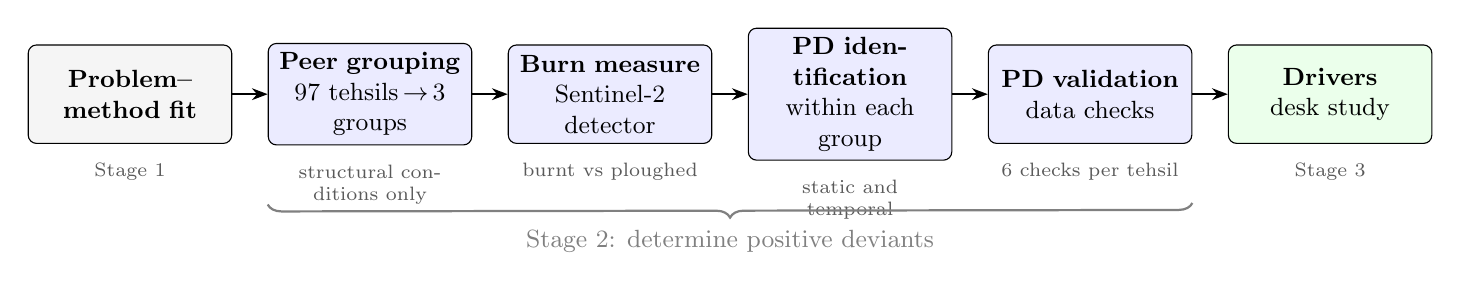
\begin{tikzpicture}[
  box/.style={draw, rounded corners=3pt, align=center, minimum height=1.25cm, text width=2.35cm, font=\small, fill=#1},
  box/.default={gray!8},
  arr/.style={-{Stealth[length=2mm]}, thick},
  lab/.style={font=\scriptsize, text width=2.35cm, align=center, text=black!65}
]
\node[box] (a) {\textbf{Problem--method fit}};
\node[box=blue!8, right=0.45cm of a] (b) {\textbf{Peer grouping}\\97 tehsils\,\ra\,3 groups};
\node[box=blue!8, right=0.45cm of b] (c) {\textbf{Burn measure}\\Sentinel-2 detector};
\node[box=blue!8, right=0.45cm of c] (d) {\textbf{PD identification}\\within each group};
\node[box=blue!8, right=0.45cm of d] (e) {\textbf{PD validation}\\data checks};
\node[box=green!8, right=0.45cm of e] (f) {\textbf{Drivers}\\desk study};
\draw[arr] (a)--(b); \draw[arr] (b)--(c); \draw[arr] (c)--(d); \draw[arr] (d)--(e); \draw[arr] (e)--(f);
\node[lab, below=0.12cm of a] {Stage 1};
\node[lab, below=0.12cm of b] {structural conditions only};
\node[lab, below=0.12cm of c] {burnt vs ploughed};
\node[lab, below=0.12cm of d] {static and temporal};
\node[lab, below=0.12cm of e] {6 checks per tehsil};
\node[lab, below=0.12cm of f] {Stage 3};
\draw[decorate, decoration={brace, amplitude=5pt, mirror}, thick, black!50]
  ([yshift=-0.75cm]b.south west) -- ([yshift=-0.75cm]e.south east)
  node[midway, below=6pt, font=\small] {Stage 2: determine positive deviants};
\end{tikzpicture}
\caption{The DPPD pipeline used in this study. Grouping is done before burning is measured, so burning cannot influence the groups.}
\label{fig:pipeline}
\end{figure*}

\subsection{Peer grouping}
\label{sec:grouping}

\paragraph{Which variables.} A grouping variable must be a \emph{structural} condition: something a tehsil cannot change by its own choices, but which affects how hard it is to avoid burning. Suspected \emph{drivers} of burning, such as machine density or market access, are left out, because they are what Stage~3 must discover. Burning itself is never used. Table~\ref{tab:dims} lists the five dimensions.

\begin{table}[t]
\caption{Grouping dimensions and why each matters for burning.}
\label{tab:dims}
\small
\begin{tabularx}{\columnwidth}{@{}l >{\raggedright\arraybackslash}X@{}}
\toprule
Dimension & Why it matters \\
\midrule
Rice share (2022) & More paddy means more straw to clear in the same short window. Taken from the 10\,m paddy map, calibrated to official district totals. \\
Monsoon rainfall & Separates the dry south-west from the wetter centre; affects irrigation and crop timing. \\
Agro-ecological zone & Separates the Siwalik foothills from the plains. \\
Groundwater stress & Punjab's water law delays paddy transplanting, which delays harvest and shortens the window before wheat. \\
Soil (8 descriptors) & Affects drainage and how easily wheat can be sown into residue. \\
\bottomrule
\end{tabularx}
\end{table}

\paragraph{Distance between tehsils.} The variables mix numbers and categories, so we use Gower distance~\cite{gower1971}. Each difference becomes a score from 0 to 1: for numbers, the gap divided by the range; for categories, 0 if equal and 1 if not. Standard Gower gives every column one vote, so soil, with eight columns, would outweigh rainfall. We therefore average columns \emph{within} each dimension first, and then give each of the five dimensions an equal weight. The one hill tehsil, Dhar Kalan, is so extreme that it is left out when computing ranges and set aside as an outlier.

\paragraph{Clustering.} We use average-linkage hierarchical clustering. It starts with every tehsil alone and repeatedly merges the two closest groups. It works directly on a custom distance, does not force groups to be round or equal in size, and produces a tree that shows how groups relate.

\paragraph{Choosing and testing the groups.} We choose the number of groups using the silhouette score, which measures how much closer a tehsil is to its own group than to the next one. We ignore groups with fewer than five tehsils, since a peer group needs enough members for comparison. We then test the result in two ways:
\begin{itemize}
  \item \textbf{Stability.} We regroup a random 80\% of tehsils 300 times and compare each result with the full grouping using the adjusted Rand index (ARI)~\cite{hubert1985ari}, where 1 means identical. Each tehsil's final group is the one it falls into most often.
  \item \textbf{Sensitivity.} We change one design choice at a time (each weight $\times$0.85 or $\times$1.15, or dropping a dimension) and measure how much the groups move.
\end{itemize}

\subsection{Burn measurement}
\label{sec:measure}

\paragraph{The problem.} A standard burn index (BAIS2~\cite{filipponi2018bais2} plus Tasseled Cap brightness) finds burnt fields well: 95.5\% accuracy on expert-labelled fields~\cite{ceew2026patterns}. But it cannot tell ash from freshly ploughed soil. On Walker et al.'s field data, it flags 98\% of burnt fields and also 81\% of ploughed fields that were never burnt. Fresh ash is near-black for only two to three days and then fades toward the colour of ploughed soil, and Sentinel-2 often misses those days because it revisits every five days.

\paragraph{The detector.} We use a two-stage approach for each field or sample point:
\begin{enumerate}
  \item \textbf{Flag.} Score every clear Sentinel-2 image with the burn index. A positive score marks a possible event (burnt or ploughed).
  \item \textbf{Pick the event.} Take the flagged image with the largest jump in score from the previous clear image. Burning is sudden, while crop drying is gradual.
  \item \textbf{Check.} Compare that image with the clear image before it (bands and indices, before and after). A random forest trained on Walker et al.'s burnt and ploughed fields~\cite{walker2024data} decides ``burnt'' or ``not burnt''. We use a cut-off of 0.79, which keeps 90\% of known burns.
\end{enumerate}
We chose a strict cut-off because ploughing false alarms are the bigger threat to DPPD: they would hide exactly the tehsils that plough instead of burning.

\paragraph{Independent check.} We tested the detector, without retraining, on fields in Jalandhar in 2021: a new year and district. Two judges were used: CEEW's expert labels from 29 October~\cite{ceew2026patterns}, and daily 3\,m PlanetScope images~\cite{planet2026}, in which a field counts as burnt if its brightness drops sharply below its recent level.

\paragraph{From fields to tehsils.} Each tehsil has a fixed panel of 100 random points that are paddy in both the 2020 and 2022 rice maps. The same points are read every season from 15 September to 30 November. A tehsil's \emph{burnt share} is the number of burnt points divided by the number of points with a verdict. We rank the 81 plains tehsils (Central and South-west). The 15 Foothills tehsils are measured but not ranked, because there the ash-versus-soil confusion is large relative to real burning.

\subsection{Identifying positive deviants}
\label{sec:pd}

We look for two kinds of deviance, always compared within a tehsil's own group:
\begin{itemize}
  \item \textbf{Static:} burns the least on average over 2020--2024.
  \item \textbf{Temporal:} reduced burning the fastest over the same period. Comparing a tehsil with its own past cancels out fixed differences we cannot measure.
\end{itemize}
\emph{Negative deviants} (NDs) are the mirror image and serve as the contrast group.

We use the handbook's outlier rule~\cite{dppd2021handbook}: a tehsil is a deviant if it lies below $Q_1 - 1.5\times\mathrm{IQR}$ of its group. Burnt share cannot go below zero, so on the raw scale this fence falls below zero and no tehsil could ever qualify. We therefore apply the rule to $\log(\text{burnt share} + c)$, where $c$ is 10\% of the group median. On this scale, halving burning counts the same at any level. A static PD must also be in its group's lowest quarter in at least four of five seasons, so one lucky season is not enough. For trends we use the Theil--Sen slope, which is robust with only five points. A \emph{strict} PD must pass the fence both on 2020--24 and on 2020--23, because 2024 behaves differently from other seasons (\S\ref{sec:res-measure}).

\subsection{Validating positive deviants}
\label{sec:validation}

The handbook asks for a check that each deviant is a real signal, not noise or an artefact~\cite{dppd2021handbook}. We ran six data checks on every candidate, with thresholds fixed in advance (Table~\ref{tab:checks}). A tehsil that fails any check is dropped. One warning is allowed for a \emph{validated PD}; more warnings make it a \emph{PD with caveat}.

\begin{table}[t]
\caption{Validation checks applied to every candidate PD.}
\label{tab:checks}
\small
\begin{tabularx}{\columnwidth}{@{}l >{\raggedright\arraybackslash}X@{}}
\toprule
Check & Question asked \\
\midrule
V1 Bootstrap & Is the flag luck in which 100 points were drawn? (1,000 resamples; pass if kept $\geq$80\%) \\
V2 Settings & Does it hold with another cut-off, offset and grouping? \\
V3 Clouds & Do cloud gaps hide fires? \\
V4 Rice & Does the tehsil simply grow less paddy? \\
V4b Harvest & Does it still burn less on points where a paddy harvest is actually seen? \\
V5 Timing & Is harvest so late that burning falls outside the window? \\
V6 Other sensors & Do VIIRS fire counts and official district figures agree? \\
\bottomrule
\end{tabularx}
\end{table}

\subsection{Discovering drivers}
\label{sec:drivers}

DPPD normally confirms what deviants do through fieldwork. Because this project used only public data, Stage~3 is a desk study, which the handbook allows when fieldwork is not possible~\cite{dppd2021handbook}. Its aim is to produce candidate explanations for a later field study, not to prove causes.

A driver is something that could, in principle, be changed or transferred. We listed nine candidate drivers from the literature and news, and could test eight with public data (Table~\ref{tab:drivers}). The ninth, CRM machines and hiring centres, could not be tested because no district-level figures are published online.

\begin{table}[t]
\caption{Candidate drivers and why each might lower burning.}
\label{tab:drivers}
\small
\begin{tabularx}{\columnwidth}{@{}l >{\raggedright\arraybackslash}X@{}}
\toprule
Driver & Reasoning (source) \\
\midrule
Harvest-to-sowing days & More time to manage straw (Sentinel-2) \\
Early second crop & Potato or vegetables sown in October need clearing without fire (Sentinel-2) \\
Farm labour, farm size & Labour for manual handling; small farms afford fewer machines (Census 2011) \\
Straw buyers & A buyer makes burning a lost sale (news reports) \\
Distance to state border & Smoke drifting to another state draws less enforcement~\cite{dipoppa2024bureaucrat} \\
Urban surroundings & Smoke is noticed; off-farm work; local markets (GHS-SMOD) \\
Basmati share & Basmati straw is fed to cattle (APEDA, district) \\
Livestock & Straw used as fodder (Livestock Census 2019) \\
\bottomrule
\end{tabularx}
\end{table}

All comparisons are made inside the peer groups in three ways: (1) whether PDs and NDs fall on the expected sides of the group median; (2) the Spearman correlation between the driver and burning across all tehsils in the group; and (3) the same correlation with rice share held constant. The last step matters because, even within groups, burning rises with rice share; a driver that only stands in for ``less paddy'' would otherwise look important. With 8 PDs and 4 NDs the analysis is descriptive, so we rely only on patterns that repeat across all three readings.

%% ===================================================================
\section{Results}
\label{sec:results}

\subsection{Three peer regions}
\label{sec:res-groups}

The method produced three groups and one outlier (Figure~\ref{fig:groups}, Table~\ref{tab:groups}). Location was never given to the method, yet the groups form three connected regions that match Punjab's known agricultural belts: the central plains, the dry Malwa south-west and the Kandi foothills. This is strong evidence that the grouping captures real structure.

\begin{figure}[t]
\centering
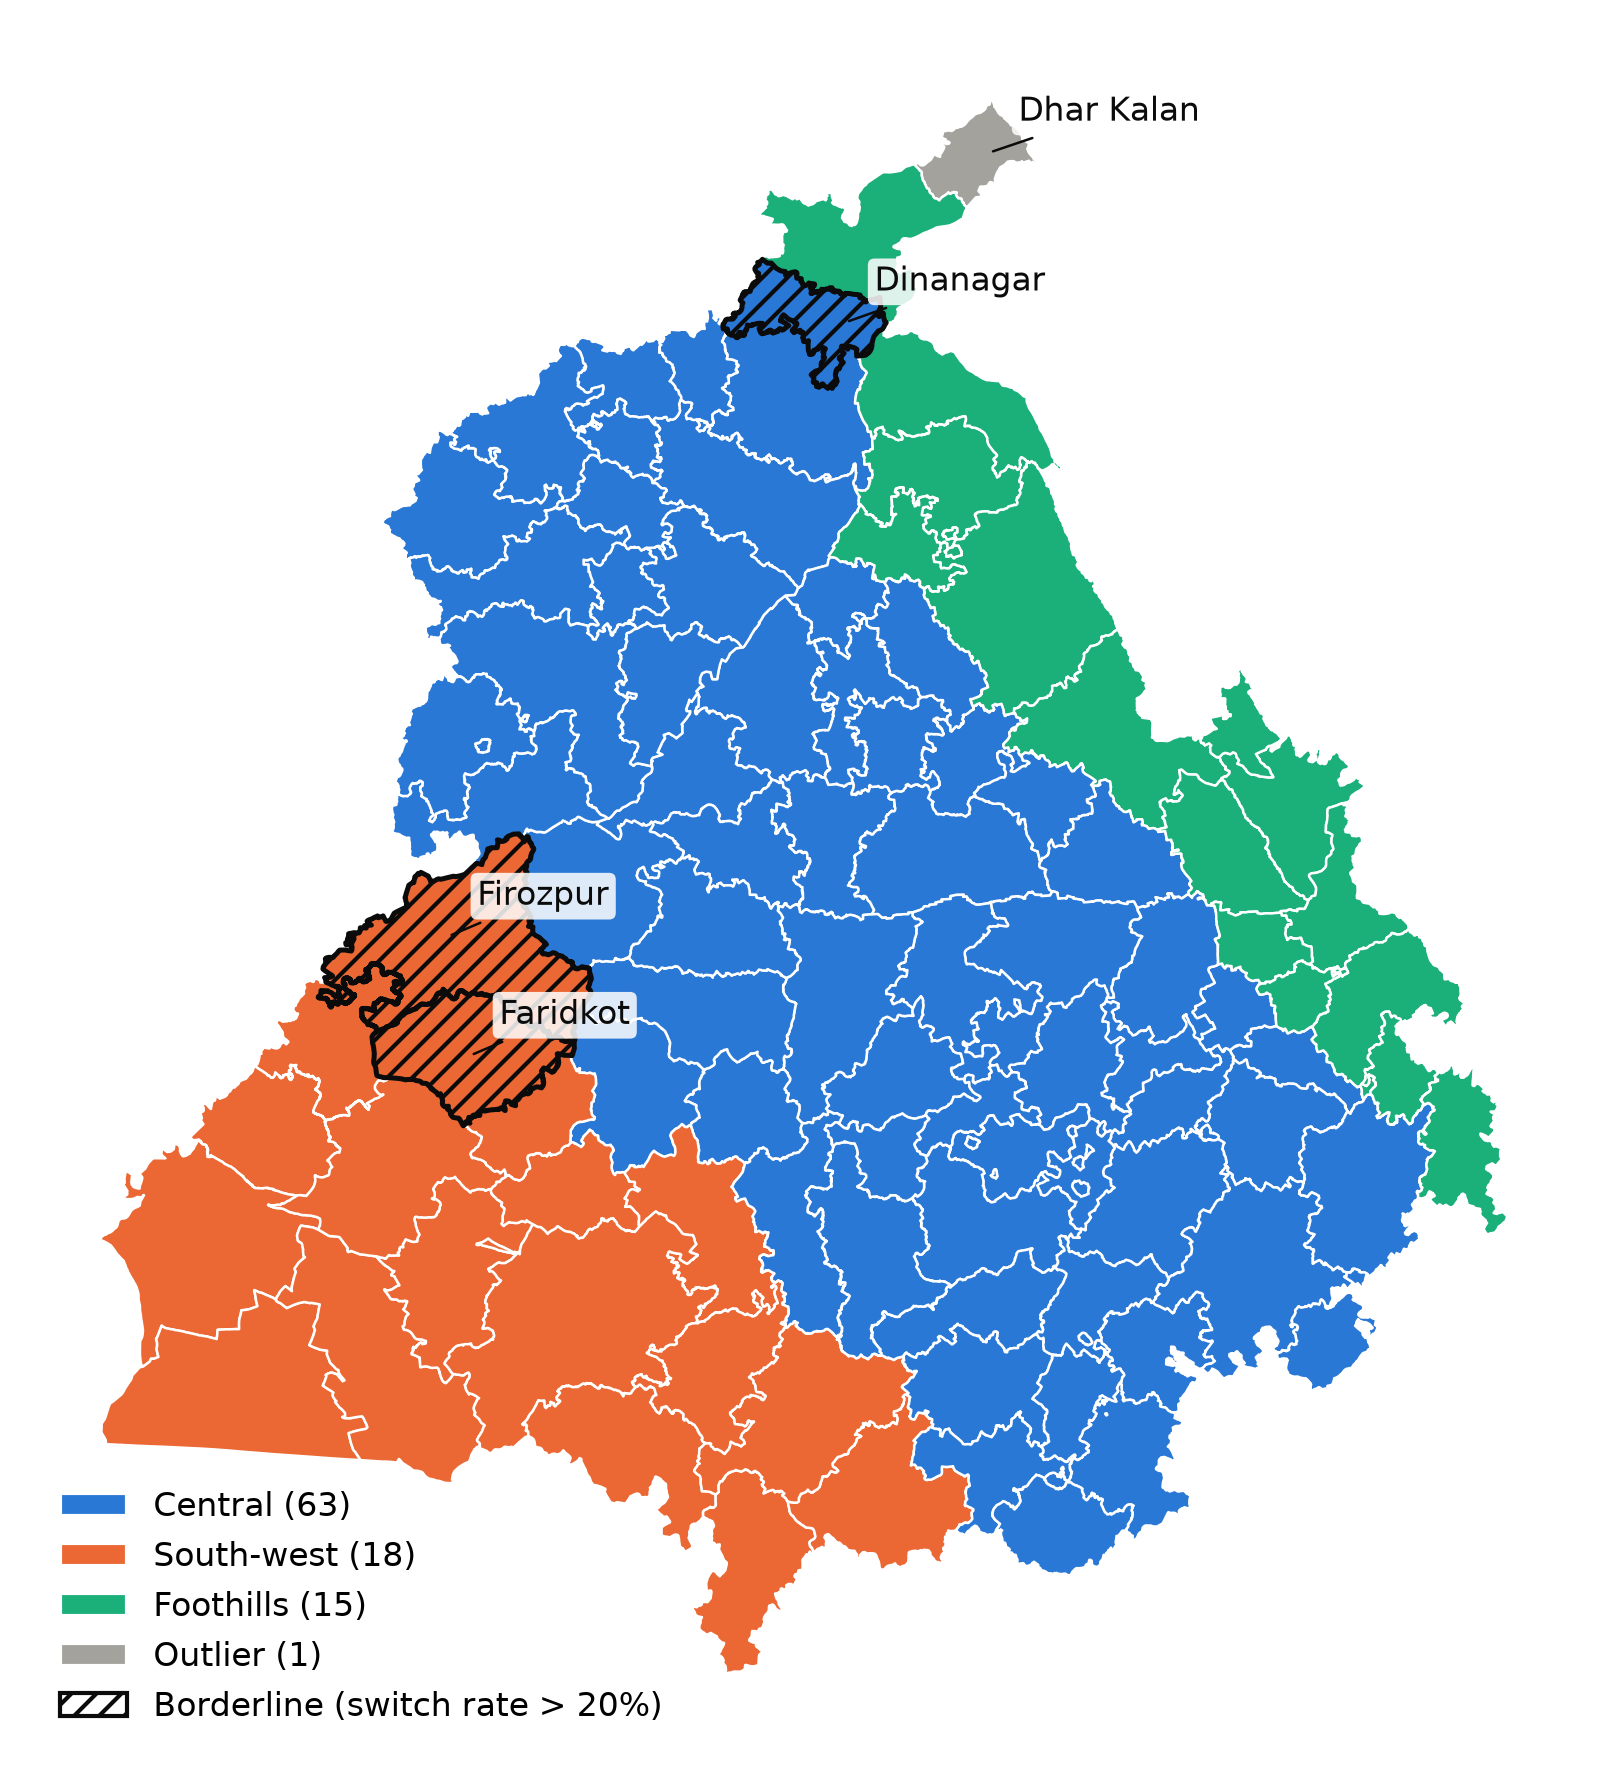
\includegraphics[width=0.92\columnwidth]{fig_groups.png}
\caption{Peer groups of Punjab's 97 tehsils. Hatched tehsils are borderline (they switch group in more than 20\% of resamples).}
\label{fig:groups}
\end{figure}

\begin{table}[t]
\caption{The three peer groups (medians). Rice = rice share of tehsil area; Rain = June--September rainfall; Groundwater = extraction as \% of annual recharge.}
\label{tab:groups}
\small
\setlength{\tabcolsep}{4pt}
\begin{tabular}{@{}lrrrr@{}}
\toprule
Group & Tehsils & Rice & Rain (mm) & Groundwater \\
\midrule
Central & 63 & 75\% & 721 & 230\% \\
South-west & 18 & 59\% & 467 & 118\% \\
Foothills & 15 & 28\% & 981 & 117\% \\
Outlier (Dhar Kalan) & 1 & 7\% & 1,604 & 27\% \\
\bottomrule
\end{tabular}
\end{table}

The grouping is stable. The silhouette score is 0.377 and the mean bootstrap ARI is 0.89. The Central and Foothills groups reappear in every resample, and the South-west in 94\%. Only three tehsils are borderline. Ten of twelve weight changes keep ARI at or above 0.83. The weak point is the South-west/Central boundary: dropping any dimension merges the two. The South-west is real, since rainfall, zone and groundwater all separate it, but it shades gradually into the centre. We therefore keep three groups and also require every PD to hold under a two-group version.

\subsection{The detector separates burning from ploughing}
\label{sec:res-detector}

On Walker et al.'s data (5-fold cross-validation), the new detector keeps 90\% of burns while cutting ploughed fields wrongly called burnt from 81\% to 18\% (Figure~\ref{fig:detector}). Its AUC is 0.94. A Sentinel-2 model trained only on PlanetScope-derived labels came close (22\% false alarms), which shows that daily imagery can stand in for field surveys when training such a model.

\begin{figure}[t]
\centering
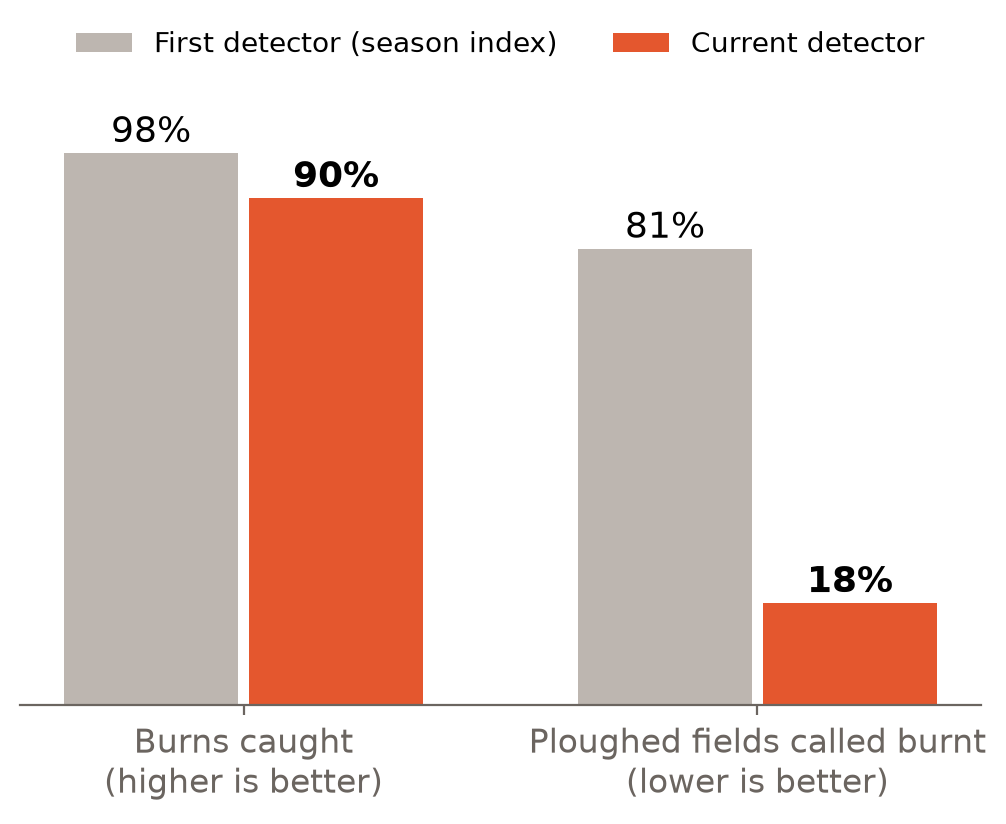
\includegraphics[width=0.8\columnwidth]{fig_detector.png}
\caption{Old season-long burn index versus the new detector, on field-verified burnt and ploughed fields from 2019.}
\label{fig:detector}
\end{figure}

On the independent Jalandhar 2021 test, false alarms fell from 23 of 32 fields to between 0 and 3 depending on the cut-off. The cost is missed burns, mostly on partly burnt fields. For ranking tehsils, missing some burns does less harm than counting ploughing as burning, as long as the misses are similar across tehsils.

\subsection{A tehsil burn measure that ranks well}
\label{sec:res-measure}

Almost every sample point gets a verdict (at least 70 of 100 in any tehsil and season). Three checks support using the measure to rank tehsils:
\begin{itemize}
  \item It ranks tehsils like an independent sensor: Spearman $\rho$ with VIIRS fire counts is 0.78--0.87 for 2019--2023.
  \item It is stable: each season's ranking agrees with the next at $\rho$ 0.82--0.91 from 2019 to 2023.
  \item The cut-off changes the level of burning but hardly the order ($\rho$ 0.84--0.98 between cut-offs 0.5 and 0.79).
\end{itemize}
The two measures agree on the order of tehsils but not on the overall trend. From 2021 to 2023, VIIRS fire counts fell by 60\%, while the share of paddy burnt fell only from 64\% to 52\% (Figure~\ref{fig:viirs}). This is consistent with farmers timing fires to avoid the satellite pass, which makes a field-level measure more valuable.

The 2024 season is unusual: 72\% of burns are first seen in late November, and agreement with VIIRS drops to 0.51. These late detections may include ploughing and sowing. We therefore leave 2024 out of Figure~\ref{fig:viirs}, and every PD result is also checked without it.

\begin{figure}[t]
\centering
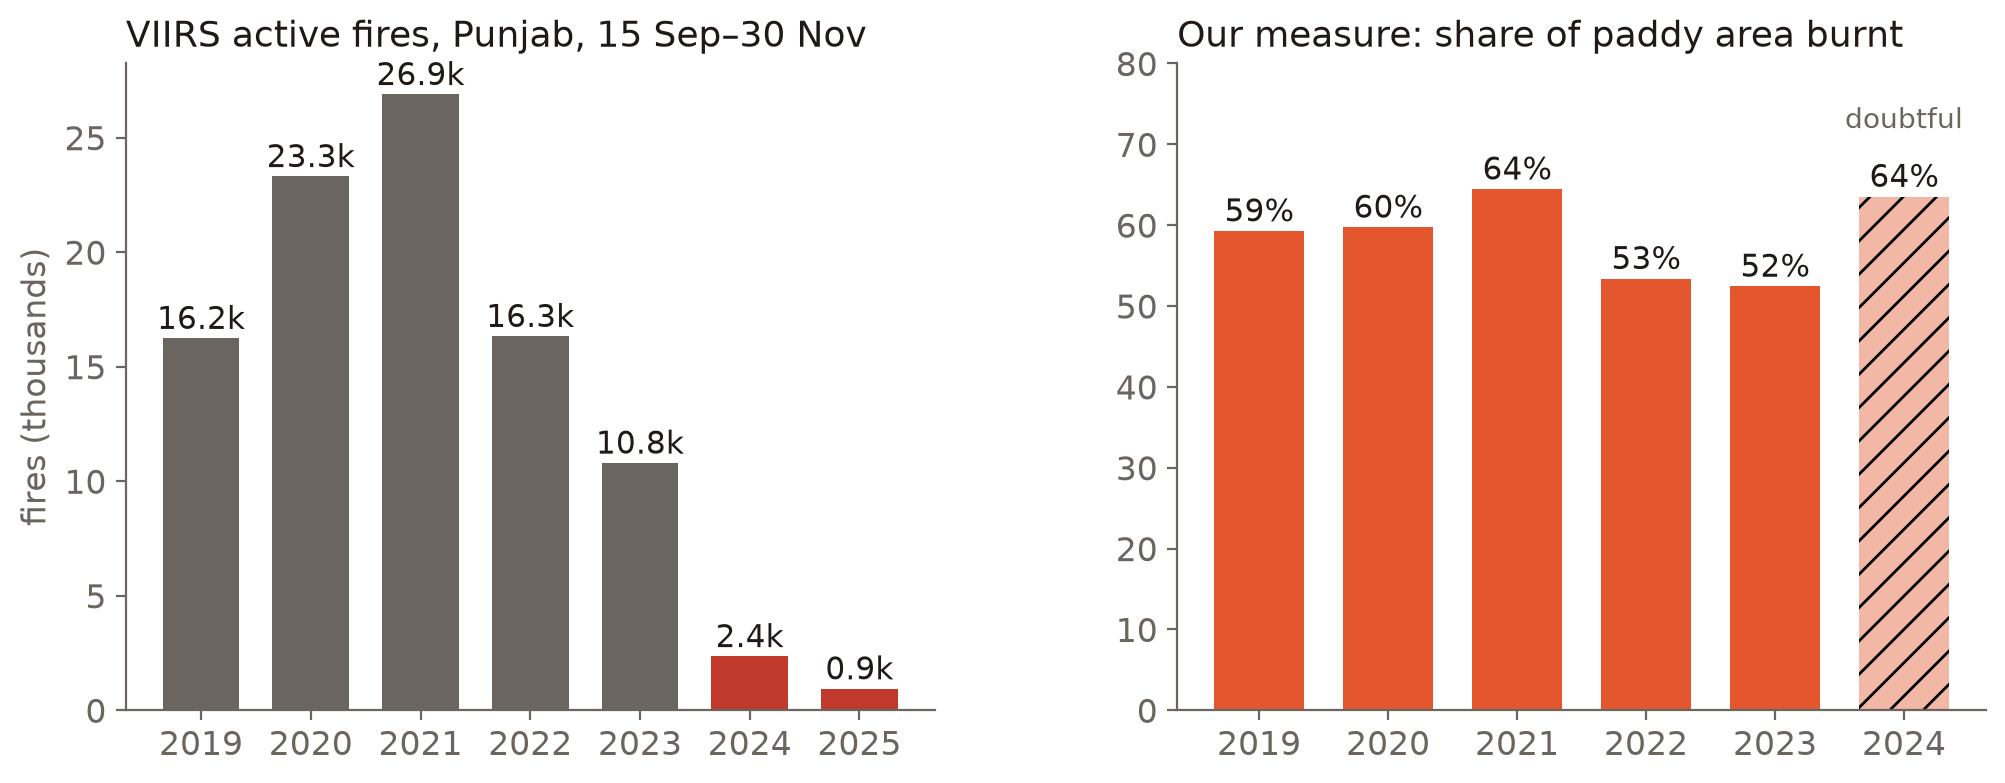
\includegraphics[width=\columnwidth]{fig_viirs.png}
\caption{VIIRS fire counts in Punjab (left) and our field-level share of paddy burnt (right), 2019--2023. Fire counts fell much faster than the burnt share.}
\label{fig:viirs}
\end{figure}

\subsection{Positive deviants}
\label{sec:res-pd}

Table~\ref{tab:pds} and Figure~\ref{fig:pdmap} show the final list.

\begin{table}[t]
\caption{Positive deviants after validation. Burnt share is the 2020--24 mean. Group medians: Central 0.62, South-west 0.73.}
\label{tab:pds}
\small
\setlength{\tabcolsep}{4pt}
\begin{tabular}{@{}llrl@{}}
\toprule
Tehsil & Group & Burnt share & Result \\
\midrule
\textbf{Abohar} & SW & 0.34 & \textbf{Strict PD} (static + temporal) \\
Dinanagar & C & 0.21 & Validated PD \\
Phagwara & C & 0.30 & Validated PD \\
Adampur & C & 0.30 & Validated PD \\
Jalandhar-I & C & 0.31 & Validated PD \\
Talwandi Sabo & SW & 0.50 & Validated PD \\
Gurdaspur & C & 0.29 & PD with caveat \\
Banga & C & 0.34 & PD with caveat \\
\midrule
\multicolumn{4}{@{}l}{\emph{Negative deviants (contrast):} Lehra, Zira, Moonak (C); Guruharsahai (SW)} \\
\bottomrule
\end{tabular}
\end{table}

\begin{figure}[t]
\centering
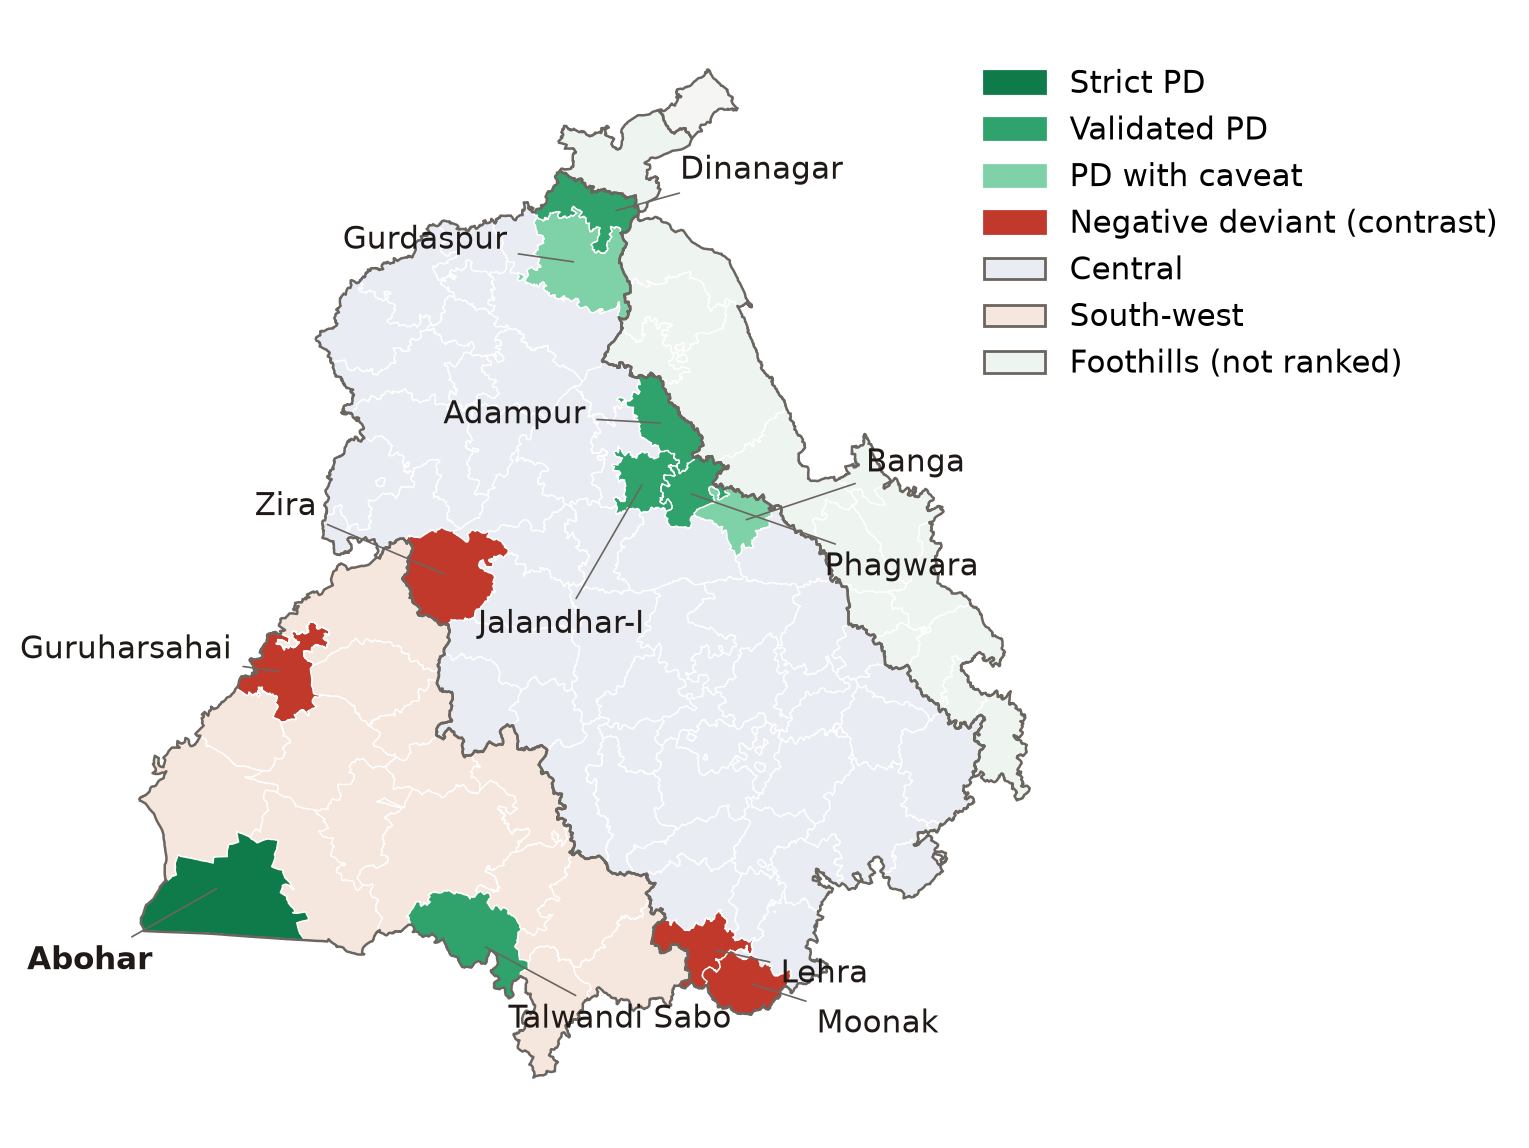
\includegraphics[width=\columnwidth]{fig_pd_map.png}
\caption{Positive and negative deviant tehsils. The Doaba PDs sit together in the north; Abohar is in the far south-west.}
\label{fig:pdmap}
\end{figure}

\paragraph{Abohar is the clearest positive deviant.} It is the lowest burner in the South-west, passes the fence in both season windows, and is among the fastest to reduce burning (11\% per year faster than its group). It is the only tehsil that is a deviant on both measures.

\paragraph{The Doaba belt burns half as much as Central Punjab.} Dinanagar, Phagwara, Adampur and Jalandhar-I (with Gurdaspur and Banga) burn about half the Central median. They lie next to each other in the Doaba region, the land between the Beas and Sutlej rivers. Six of the eight static PDs were also flagged by VIIRS fire counts, so the list does not depend on one sensor.

\paragraph{Validation.} The static list holds up. Every validated PD keeps its flag in at least 89\% of bootstrap resamples and under three or four of the four alternative settings. Temporal deviance, however, does not hold up except for Abohar: the two other fast reducers (Samana and Dirba) kept their flag in only about 40\% of resamples and were dropped. A five-season trend from 100 points per tehsil is too noisy to name a deviant on its own.

\paragraph{The rice question.} Most PDs grow less rice than their peers, and across all tehsils burning rises with rice share even inside a group ($\rho$ 0.70 in Central, 0.63 in South-west; Figure~\ref{fig:rice}). Is low burning just ``less paddy''? Check V4b says no. When we score only points where a paddy harvest was actually seen, PDs still burn far less than their groups (Abohar 0.45 against a group median of 0.73; Dinanagar 0.25 against 0.62). The PDs burn little on fields that really grew paddy.

\begin{figure}[t]
\centering
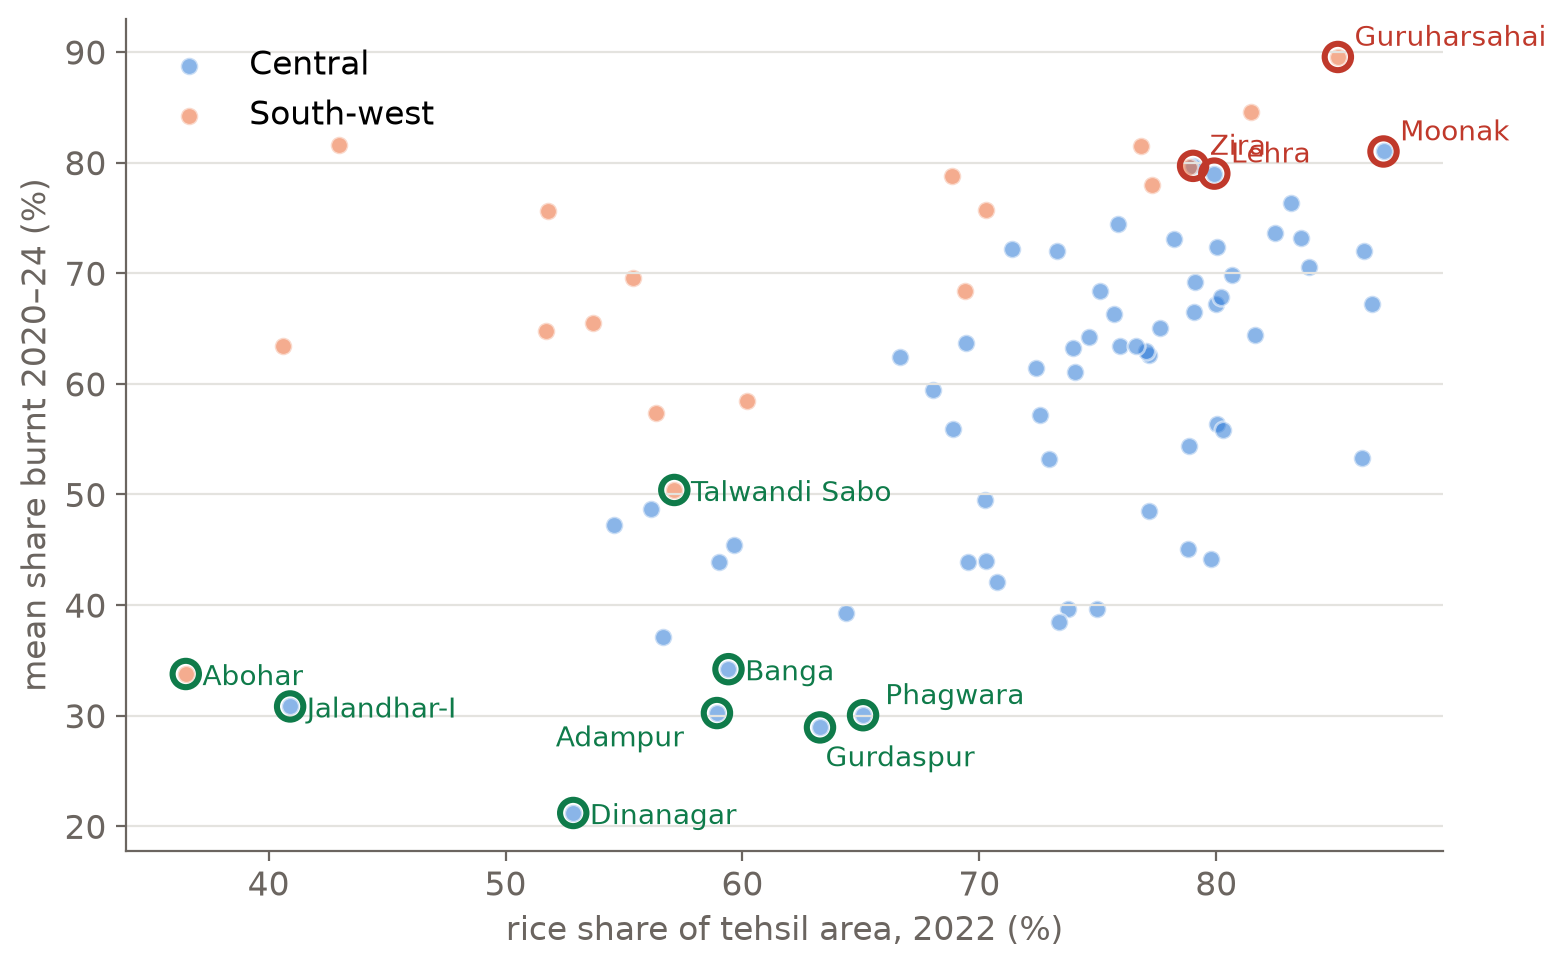
\includegraphics[width=\columnwidth]{fig_rice.png}
\caption{Burning against rice share. Burning rises with rice share, but the PDs (green) burn less than tehsils with similar rice share.}
\label{fig:rice}
\end{figure}

\subsection{What might explain the deviants}
\label{sec:res-drivers}

Figure~\ref{fig:drivers} summarises how each driver relates to burning in the Central group, before and after holding rice share constant. Four findings stand out.

\begin{figure*}[t]
\centering
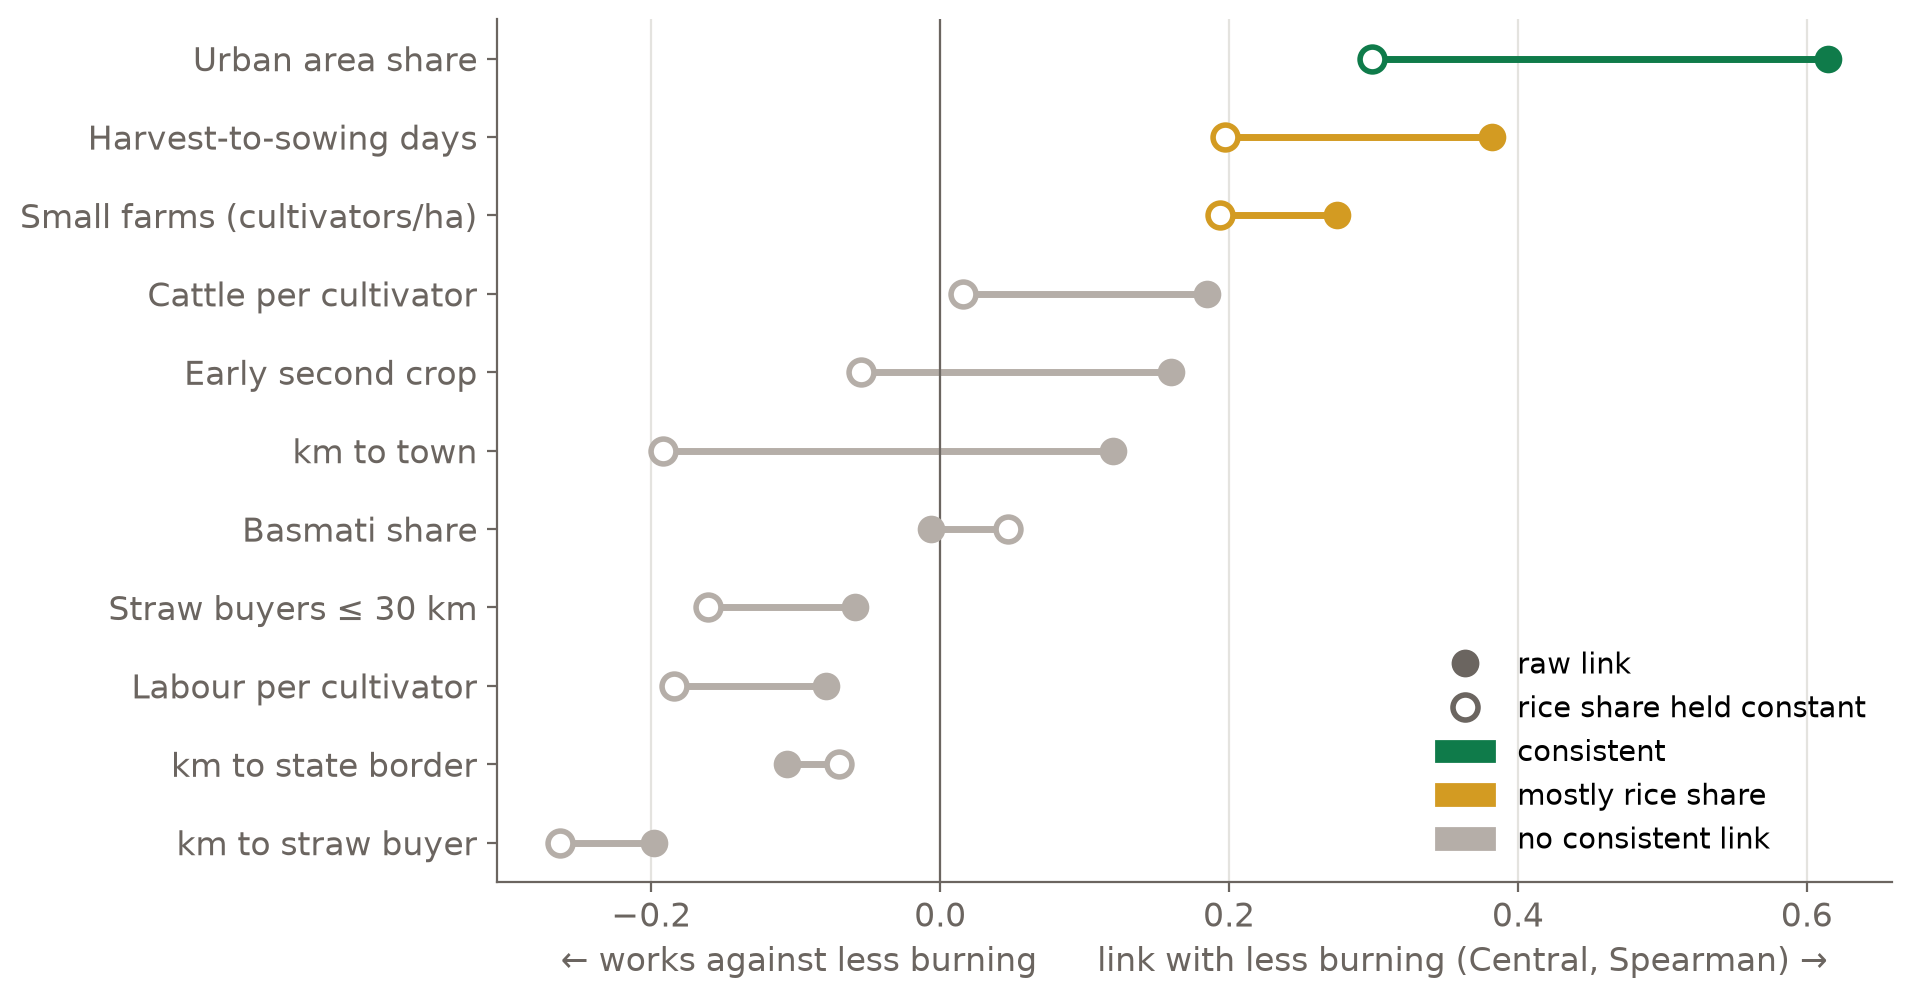
\includegraphics[width=0.72\textwidth]{fig_drivers.png}
\caption{How each driver relates to lower burning in the Central group (Spearman). Filled dot: raw link. Open dot: with rice share held constant.}
\label{fig:drivers}
\end{figure*}

\paragraph{1. Urban surroundings mark the Doaba belt as a region.} Urban area share is the only driver consistent on all three readings in Central. Seven of eight PDs have more urban land than their group median, and all four NDs have less ($\rho = -0.61$; $-0.30$ with rice share held constant). But the effect is not about being near a town. Within tehsils, fields more than 2\,km from a town show no difference by distance, and PDs still burn as little when scored only on fields more than 5\,km from any urban centre (for example, Dinanagar 0.21 \ra\ 0.20, Adampur 0.30 \ra\ 0.30). Urban share is best read as a marker of the Doaba region and what comes with it: potato and vegetable rotations, off-farm and overseas incomes, and dense markets.

\paragraph{2. Abohar has a distinct profile.} Abohar is rural, yet it stands out on several drivers at once: a biomass power plant inside the tehsil (a local straw buyer)~\cite{ht2017biomass}, the most farm labourers per cultivator in Punjab, the most cattle and buffalo per cultivator in its group, and the highest share of early second crops in its group. Each is a plausible route to less burning. With one tehsil they cannot be separated, so this is a lead for fieldwork.

\paragraph{3. Some apparent drivers are really rice share.} A longer harvest-to-sowing gap and smaller farms both seem linked to less burning, but most of the link disappears once rice share is held constant. Where paddy dominates, harvest and sowing are more crowded and farms differ, so these variables mostly restate the rice gradient.

\paragraph{4. No consistent link for the rest.} Straw buyers within 30\,km, labour per cultivator, district basmati share and livestock showed no consistent pattern. Some of these data are coarse (district-level basmati, a town-level buyer list), so these are weak tests rather than evidence of no effect.

%% ===================================================================
\section{Discussion}
\label{sec:discussion}

\paragraph{What this means for NGOs and government.}
\begin{itemize}
  \item \textbf{Where to look.} Field teams should start in Abohar and the Doaba belt, with the high-burning NDs as the comparison. A small field study there costs far less than a statewide survey.
  \item \textbf{What to test.} Abohar suggests three levers that could be tried elsewhere in the South-west: an assured local straw buyer, paid labour for straw handling, and links to fodder demand. For Doaba, the open question is what farmers do with straw before an October potato or vegetable crop.
  \item \textbf{How to rank places fairly.} Programmes that rank districts or tehsils by burning should compare like with like and allow for rice share. Otherwise they reward places that simply grow less paddy.
  \item \textbf{How to monitor.} Fire counts are becoming less reliable as farmers avoid the satellite pass. A free, field-level Sentinel-2 measure that separates burning from ploughing can be rerun every season.
\end{itemize}

\paragraph{Lessons for the DPPD method.}
\begin{itemize}
  \item \textbf{Audit the data first.} Several widely used datasets had serious problems for Punjab. The 10\,m paddy map over-maps rice in the south-west by up to 1.7 times, so we calibrated it to official district totals. Our satellite cropping-intensity estimate barely agreed with official figures ($\rho$ = 0.18) and was dropped. Terrain data had defective slope values and was replaced by agro-ecological zones.
  \item \textbf{Group before measuring.} Building groups without knowing the outcome removes any chance of shaping them to produce deviants.
  \item \textbf{Adapt the outlier rule to the data.} For a share that cannot go below zero, the standard fence fails on the raw scale. A log scale fixes this.
  \item \textbf{Static deviance is more robust than temporal deviance} when the sample per unit is small. Trends need more points or more seasons.
  \item \textbf{Deviants may form regions.} The Doaba PDs sit together, so the fence counts much of the cluster as normal spread. Clusters of low performers deserve attention, not just isolated outliers.
\end{itemize}

%% ===================================================================
\section{Impact Assessment Plan}
\label{sec:impact}

DPPD stops at candidate explanations. The next step is to check them and test whether they transfer~\cite{dppd2021handbook}. We propose a two-phase plan that a partner organisation could run.

\paragraph{Theory of change.} PD leads (this study) \ra\ confirm in the field what PDs do differently \ra\ pilot the confirmed levers in similar non-PD villages \ra\ measure the change in burning by satellite and survey \ra\ scale up if the effect holds.

\paragraph{Phase 1: field validation (one season).} Visit Abohar, the four Doaba PDs and the four NDs. In each tehsil, pick about six villages across the range of satellite burnt share. Activities: a farmer survey (about 20 rice farmers per village), one focus group per village, interviews with block officers, straw buyers and hiring-centre operators, and dated, geotagged photos of sample points at harvest to give the detector a field-located check. Only levers confirmed here move to Phase~2.

\paragraph{Phase 2: matched, randomised pilot.} For the Abohar-derived levers (straw buyer, labour, fodder link), sample villages in non-PD tehsils of the South-west group. The peer groups are what make treated and control villages comparable; this is the main thing DPPD adds to a standard pilot. Pair villages on past burnt share and rice share, and randomly assign one village in each pair to receive the lever. Controls are drawn at least one village away, and neighbouring villages are tracked to catch spillovers.

\paragraph{Outcomes.} The primary outcome is each village's burnt share from our Sentinel-2 detector. It covers every field, needs no interview and already has a five-season baseline. Secondary outcomes come from a survey: reported burning, wheat sowing date, straw-management cost and wheat yield. Because burning is illegal, the survey asks about it through a \emph{list experiment}: farmers report only how many statements on a list are true, so no one has to admit burning directly.

\paragraph{Sample size.} Using our measure's variation across South-west tehsils and its year-to-year stability, detecting a 10-point drop in burnt share (about one-sixth of current burning) at 80\% power needs about 30 villages per arm in our central scenario, scoring at least 30 points per village. We recommend 35 pairs (70 villages) per lever to allow for villages where the lever is not delivered. This fits easily within the 1,633 villages of the South-west frame.

\paragraph{Ethics.} Ethics approval and informed consent in Punjabi come first. Answers about burning are never stored with names or plot locations, and satellite results are reported only at village level or above, so they cannot be used against individual farmers. The pilot only adds options; no existing scheme is withheld from control villages.

%% ===================================================================
\section{Limitations}
\label{sec:limitations}

\begin{itemize}
  \item \textbf{No fieldwork.} This was an academic study using only public data. No practice is confirmed on the ground, and no PD point was checked visually or in the field.
  \item \textbf{Detector validation is limited.} Ploughing is tested only on Walker et al.'s data (one season, two districts). The detector misses about half of partly burnt fields.
  \item \textbf{Sample size per tehsil.} 100 points per tehsil is enough for ranking, but not for five-season trends.
  \item \textbf{Uncertain 2024 season,} and the 15 Foothills tehsils are measured but not ranked.
  \item \textbf{Grouping inputs.} Rice share uses one year with district-level calibration, rainfall uses a five-year mean, soil has about one sample per 2011 tehsil, and temperature was not included. Equal weights are a design choice that the South-west boundary is sensitive to.
  \item \textbf{Driver data.} Stage~3 rests on 8 PDs and 4 NDs and on data from different years (2011--2023). District-level data on CRM machines was not available online.
  \item \textbf{Scope.} Only Punjab was studied. Haryana was left out because its groundwater, crosswalk and soil data are incomplete.
\end{itemize}

%% ===================================================================
\section{Conclusion}

We built an end-to-end, reproducible DPPD pipeline for crop residue burning, from public data to a validated list of positive deviant tehsils and candidate explanations. Peer groups built only from structural conditions turned out stable and matched Punjab's known agricultural regions. A two-stage Sentinel-2 detector removed most of the ploughing false alarms that affect season-long burn indices. Within these groups, Abohar stands out as the clearest positive deviant, and the Doaba belt burns about half as much as the rest of Central Punjab, on fields that really grew paddy. Several commonly cited explanations, such as a short harvest-to-sowing window and small farms, turned out mostly to reflect how much paddy a place grows.

These results are leads, not causal claims. They tell field teams where to look first and which levers to test: an assured straw buyer, farm labour and fodder demand in the South-west, and the Doaba crop rotation. With field access, more daily imagery and district machine data, the same pipeline can give firmer answers and can be rerun every season.

\begin{acks}
We thank Prof.\ Aaditeshwar Seth for supervising this project, and Basma Albanna and Andreas Pawelke of the DPPD initiative for their guidance on the method. PlanetScope imagery was provided by Planet Labs PBC through its Education and Research Program. We thank the authors of the public datasets used here, in particular Walker et al.\ and CEEW for releasing their field data.
\end{acks}

\bibliographystyle{ACM-Reference-Format}
\bibliography{references}

%% ===================================================================
\appendix

\section{Data Problems and How We Solved Them}
\label{app:problems}

Many of the hardest parts of this project were data problems rather than modelling problems. We record them because they affect how far the results can be trusted, and because others using the same public data for Punjab will meet them too.

\begin{table}[h]
\caption{Main data problems and how each was handled.}
\label{tab:problems}
\small
\begin{tabularx}{\columnwidth}{@{}>{\raggedright\arraybackslash}p{0.46\columnwidth} >{\raggedright\arraybackslash}X@{}}
\toprule
Problem & How we handled it \\
\midrule
Most data use 2011 Census units, but many current tehsils were carved out of old ones. & Built village- and tehsil-level crosswalks from the Local Government Directory. \\
A village rice file's ``2022'' column was a copy of 2020. & Recomputed rice area from the 2022 paddy map over current boundaries. \\
Total rice area mostly measures tehsil size. & Used rice share (rice area / tehsil area). \\
The paddy map over-maps rice in the south-west and foothills (up to 1.7$\times$). & Calibrated it to official district rice area. \\
Satellite cropping intensity barely agreed with official figures ($\rho$ = 0.18). & Dropped; this changed only two borderline tehsils. \\
Terrain data had identical slope values across tehsils. & Replaced by agro-ecological zones. \\
The arid zone also covers 12 wetter central tehsils. & Kept rainfall alongside the zones. \\
Over a season, almost every field is flagged as burnt. & Built the two-stage detector (\S\ref{sec:measure}). \\
Sentinel-2's cloud mask labels fresh ash as ``dark area''. & Widened the mask; 436 of 438 labelled fields kept. \\
VIIRS finds about 3.7$\times$ fewer burns than Sentinel-2. & Used only as an independent cross-check. \\
The first grouping came from an AI chat session with no code. & Rebuilt the whole pipeline in code with fixed seeds. \\
\bottomrule
\end{tabularx}
\end{table}

\section{Reproducibility}

All results come from code in the project repository. Grouping scripts are in \texttt{Code/grouping/}, the burn measure in \texttt{Code/burn/}, PD identification and validation in \texttt{Code/pd/}, and the sample-size calculation in \texttt{Code/impact/}. Random seeds are fixed, and the input file hashes for the final grouping are recorded alongside its outputs.

\end{document}
